\subsection{Efficient Computation of Visibility Polygons \cite{DBLP:journals/corr/BungiuHHHK14}}
Bungiu, Hemmer, Hershberger, Huang and Kr\"oller  \cite{DBLP:journals/corr/BungiuHHHK14} introduce the implementations and their experimental evaluations for two existing algorithms (\cite{joe1987corrections}, \cite{asano1985efficient}) and a newly developed one for computing visibility in polygons. These implementations are available in the CGAL library (\url{https://www.cgal.org/}), starting with version 4.5.


Therefore, Bungiu et al. present three algorithms and their practical performance.

\subsubsection{Algorithm of Joe and Simpson \cite{joe1987corrections}}
The algorithm of Joe and Simpson \cite{joe1987corrections} runs in $O(n)$ time and space. 

Let $v_i$, for $i = {1, 2, ..., n}$, be the boundary vertices of the polygon $\mathcal P$. Let $p$ be a guard in $\mathcal P$, and let $s$ be a stack datastructure. The stack $s$ will be used to keep track of the vertices determining $Vis(p)$. 

The algorithm begins by scanning the boundaries of $\mathcal P$. The scanning is done through shooting rays $pv_i$, for $i = {1, 2, ..., n}$ in this order. The endpoints $v_i$ and $v_{i + 1}$ of each ray form a boundary edge $\overline{v_iv_{i + 1}}$. In this way, the processing of $v_i$ and $v_{i + 1}$ is done by checking whether the points are in $Vis(p)$. This means that the position of every $v_{i + 1}$ with respect to the ray $pv_i$ is checked. If $v_{i + 1}$ is found in front of the ray $pv_i$ (if $v_{i + 1}$ is seen from $p$), then both $v_i$ and $v_{i + 1}$ are added to the processing stack $s$. For every newly pushed vertex on $s$, the algorithm checks whether the segment $v_iv_{i + 1}$ obscures any of the previously added vertices. If that is the case, then the endpoints of the obscured line segment are declared obsolete and deleted. The polygon comprised of the vertices from $s$ forms at the end the visibility polygon $Vis(p)$.

% TODO: this might need better explanation? not sure if edge cases are needed
Figure \ref{fig:joe} displays an example run of the Algorithm of Joe and Simpson \cite{joe1987corrections} for polygon $\mathcal P$ and guard $p$. First, the ray from $p$ is shot through vertex $v_1$, and $v_1$ is added to $s$. Then, the ray from $p$ is shot through $v_2$. Since $pv_2$ takes a right turn from $pv_1$, this means that $v_2$ is still in the visibility region of $p$. For this reason, $v_2$ is also added to $s$. The ray passing through $v_2$ also intersects the boundary of $\mathcal P$ in a point $v_2'$. To account for the fact that $p$ can see ``behind'' $v_2$ and is still inside $\mathcal P$, the boundary vertex $v_2'$ is hence added to $s$. Next, the ray $pv_3$ takes a left turn from $v_2$, which means that $v_3$ is not seen from $p$. At the end, $Vis(p) = \{v_1, v_2, v_2', v_4, v_5, v_5', v_7, v_8, v_9, v_{10}\}$, as shown on the boundary of the green area. 

\begin{figure}[h!]
	\centering
	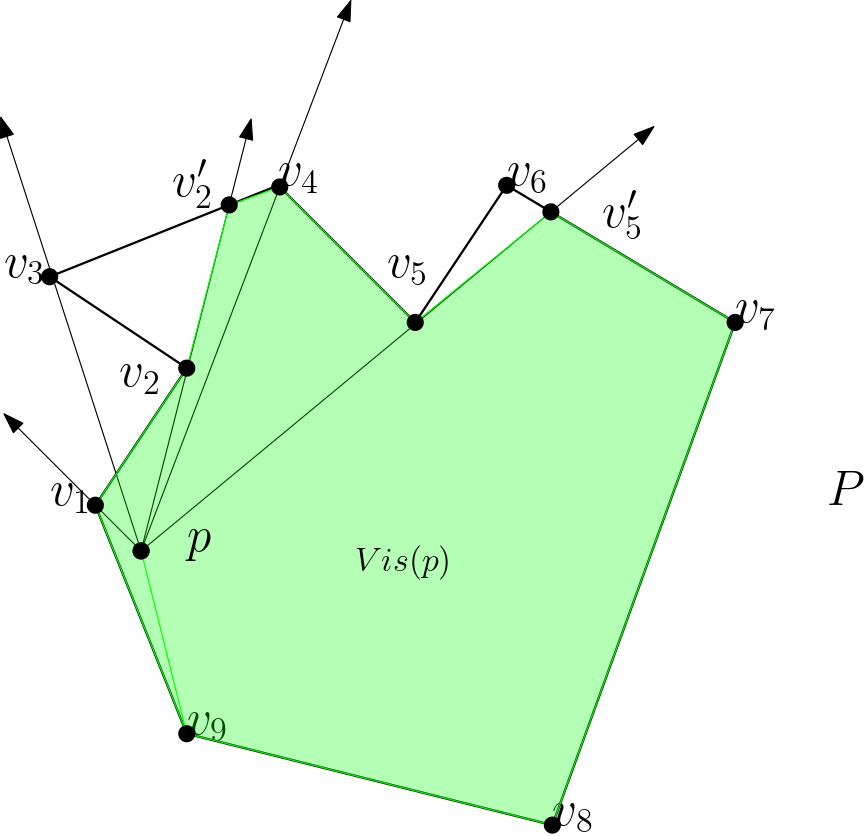
\includegraphics[width=0.4\textwidth]{joe_simpson_eg.png}
	\caption{An example run of the algorithm of Joe and Simpson \cite{joe1987corrections} for polygon $\mathcal P$ guarded by $p$ and boundary vertices $v_i$, for $i = \{1, 2, ..., n\}$.}
	\label{fig:joe}
\end{figure}

% boundaries of t	he simple polygon $\mathcal P$, and adds its boundary points $v_i, \forall i = \overline{1, n}$, with $n$ the number of vertices in $\mathcal P$, to a stack $s$. For each processed edge $\overline{v_iv_{i + 1}}$, its endpoints $v_i$ and $v_{i + 1}$ are checked whether they are in the visibility region of the viewpoint $p$. If they are, $v_i$ and $v_{i + 1}$ are added to~$s$. Otherwise, they are skipped. At every moment, the algorithm checks whether $\overline{v_iv_{i + 1}}$ obscures a previously added line segment. If that is the case, then the endpoints of the obscured line segment are declared obsolete and deleted. 

% The implementation of the algorithm handles the previously discussed cases for an arrangement $\mathcal P$, while also accounting for the case in which the polygon winds more than 360$^\circ$ using a winding counter.
% - **Algorithm of Joe and Simpson** $O(n)$ time and space
	% - performs a sequential scan of the boundary of $\mathcal P$ and uses a stack $s$ of boundary points $s_0, s_1, ..., s_ as summarised in the following subsections.der to deal with cases in which the polygon winds more than 360*, a winding counter is used during this edge processing
% he points that are visible from $q$ form the visibility region $\mathcal V(q)$ (polygon)

\subsubsection{Algorithm of Asano \cite{asano1985efficient}}
The algorithm of Asano \cite{asano1985efficient} runs in $O(n \log n)$ time and $O(n)$ space. It uses a plane sweep approach with event line $L$. 

Let $\mathcal P$ be a polygon determined by vertices $\{a_1, a_2, a_3, b_1, b_2, b_3, b_4\}$. Suppose we want to guard it by point $p$. The algorithm of Asano \cite{asano1985efficient} begins by efficiently sorting all the vertices of $\mathcal P$ based on their polar angles with respect to the guard $p$. Figure \ref{fig:asano} displays an example run of the algorithm. The points will be treated in the order of $a_2, a_1, a_3, b_4, b_3, b_2, b_1$ with respect to $p$ and their angular comparisons $$\measuredangle a_2Op < \measuredangle a_1Op < \measuredangle a_3Op < \measuredangle b_4Op < \measuredangle b_3Op < \measuredangle b_2Op < \measuredangle b_1Op,$$ where $O = (0, 0)$. 

Then, the event line $L$ starts sweeping around $p$ as shown in Subfigures \ref{fig:asano1} - \ref{fig:asano7}. Every line segment that $L$ intersects is stored in a balanced binary tree $T$ in the order of their intersection angle. As $T$ is updated, a new vertex of $Vis(p)$ is stored each time the segment closest to $p$ in $T$ changes. It is important to mention that the intersection between $L$ and line segments is not explicit, but is instead determined by comparisons between the endpoints' coordinates. For instance, in Figure \ref{fig:asano}, the endpoint $b_2$ of line segment $\overline{b_2a_2}$ is the first one $L$ intersects. Point $b_2$ is thus added to $T$. Then, $L$ continues sweeping and adds $b_1, a_2$ and $a_1$ to $T$. Although $\overline{b_2a_2}$ and $\overline{b_1a_1}$ represent line segments $s_2$ and $s_1$, respectively, the intersection of $L$ with them is not explicitly computed, but is determined based solely on the positions of their endpoints: $s_1$ is farther away from $p$ because $q, a_2$ and $b_2$ are on the same side of $s_2$.

\begin{figure}[h!]
	\centering
	\begin{subfigure}{0.45\linewidth}
		\includegraphics*[width = \linewidth]{asano7.png}
		\caption{$a_2$ is added to the empty $Vis(p)$ such \\ that $Vis(p) = \{a_2\}$.}
		\label{fig:asano1}
	\end{subfigure}
	\begin{subfigure}{0.45\linewidth}
		\includegraphics*[width = \linewidth]{asano1.png}
		\caption{$a_1$ is added to $Vis(p)$ such that \\ $Vis(p) = \{a_1, a_2\}$, and line segment $\overline{b_1a_1}$ is added to the empty binary tree $T = \{\overline{b_1a_1}\}$.}
	\end{subfigure}
	\begin{subfigure}{0.45\linewidth}
		\includegraphics*[width = \linewidth]{asano2.png}
		\caption{$a_3$ is added to $Vis(p)$ such \\ that $Vis(p)~=~\{a_1, a_2, a_3\}$,  and line \\ segment $\overline{a_1a_3}$ is added to $T$ such that \\ $T = \{\overline{b_1a_1}, \overline{a_1a_3}\}$.}
	\end{subfigure}
	\begin{subfigure}{0.45\linewidth}
		\includegraphics*[width = \linewidth]{asano3.png}
		\caption{$b_4$ is added to $Vis(p)$ such \\ that $Vis(p)=\{a_1, a_2, a_3, b_4\}$, and line \\ segment $\overline{a_3b_4}$ is added to $T$ such that \\ $T = \{\overline{b_1a_1}, \overline{a_1a_3}\, \overline{a_3b_4}\}$.}
	\end{subfigure}
\end{figure}
\begin{figure}[h!]
	\ContinuedFloat
	\centering
	\begin{subfigure}{0.45\linewidth}
		\includegraphics*[width = \linewidth]{asano4.png}
		\caption{$b_3$ is added to $Vis(p)$ \\ such that $Vis(p)=\{a_1, a_2, a_3, b_4, b_3\}$, \\ and line segment $\overline{b_4b_3}$ is added to $T$ \\ such that $T = \{\overline{b_1a_1}, \overline{a_1a_3}\, \overline{a_3b_4}, \overline{b_4b_3}\}$.}
	\end{subfigure}
	\begin{subfigure}{0.45\linewidth}
		\includegraphics*[width = \linewidth]{asano5.png}
		\caption{$b_2$ is added to $Vis(p)$ such that \\ $Vis(p) = \{a_1, a_2, a_3, b_3, b_4, b_2\}$, and line segment $\overline{b_2a_2}$ is added to $T$ such that \\ $T = \{\overline{b_1a_1}, \overline{a_1a_3}\, \overline{a_3b_4}, \overline{b_4b_3}, \overline{b_2a_2}\}$.}
	\end{subfigure}

	\begin{subfigure}{\linewidth}
		\centering
		\includegraphics*[width = 0.6\linewidth]{asano6.png}
		\caption{$b_1$ is not added to $Vis(p)$ because it is obstructed by the line segment $\overline{b_2a_2}$ which is already in $T$. For the same reason, line segments $\overline{b_3b_1}$ and $\overline{b_1a_1}$ are also not added in $T$.}
		\label{fig:asano7}
	\end{subfigure}
	\caption{Example run of the Algorithm of Asano \cite{asano1985efficient} on polygon $\mathcal P$ and guard $p$. The vertices of $\mathcal P$ are added to the binary tree $T$ in the order of their angle between $p$ and the origin $O = (0, 0)$. The result of the algorithm is visibility region $Vis(p) = \{a_1, a_2, a_3, b_3, b_4, b_2\}$.}
	\label{fig:asano}
\end{figure}



% \begin{figure}[h!]
% 	\centering
% 	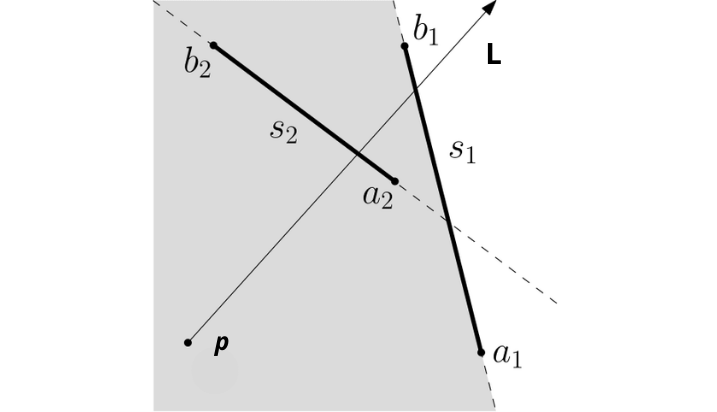
\includegraphics[width = 0.5\textwidth]{compare_segments.png}
% 	\caption{The Algorithm of Asano \cite{asano1985efficient} Visual Example \cite{DBLP:journals/corr/BungiuHHHK14}.}
% 	\label{fig:asano}
% \end{figure}
	% - as the sweep proceeds, $T$ is updated and a neq vertex of $V(q)$ is generated each time the smallest element (segment closest to $q$) in $T$ changes
	% - important to have efficient comparison ops (e.g.: *add pic*)
\newpage 
\subsubsection{New Algorithm: Triangular Expansion}
The algorithm introduced by Bungiu et al. \cite{DBLP:journals/corr/BungiuHHHK14} is named Triangular Expansion and runs in $\Omega(n^2)$ time and $O(n)$ space. It begins by triangulating $\mathcal P$ in $O(n \log n)$ time if $\mathcal P$ has holes, and $O(n)$ otherwise. The implementation runtime is constrained by CGAL, which makes use of the Delaunay triangulation algorithm \cite{delaunay1934sphere} with $O(n^2)$ time for the worst case, but with better performance in practice. 

Taken from \cite{DBLP:journals/corr/BungiuHHHK14} and annotated to suit the explanations in these summaries, Figure \ref{fig:triangular} depicts an example run of the algorithm on a polygon with holes $\mathcal P$. Starting from the viewpoint $p$, the triangle containing $p$ is located by performing a simple walk. Trivially, $p$ sees the entire triangle it is contained in. The algorithm continues by recursively expanding the view of $p$ from one triangle into the next, until there are no more triangles to expand into. The view of $p$ becomes restricted by the reflex vertices $l$ and $r$ of the third triangle entered by the recursive step. Since $l$ and $r$ are reflex vertices, the view past them is further restricted until the boundaries $l'$ and $r'$ of $\mathcal P$, respectively,  are reached. Line segments $\overline{ll'}$ and $\overline{rr'}$ are added to $Vis(p)$ in their angular order around $p$. At the end, $Vis(p)$ will contain the segments delimiting the visibility polygon of $p$.

\begin{figure}[h!]
	\centering
	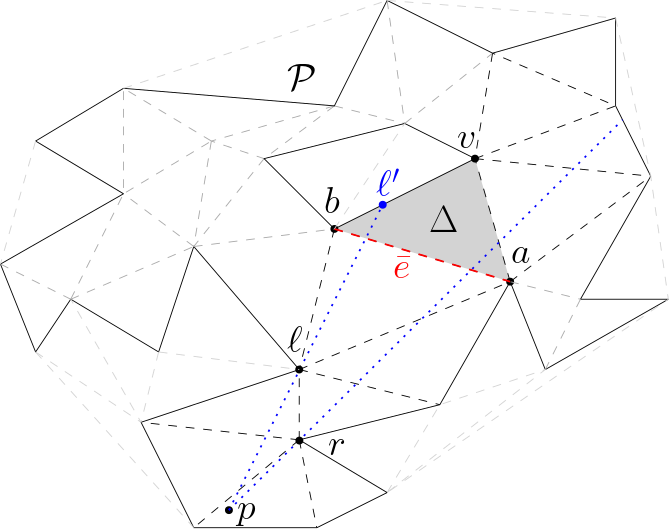
\includegraphics[width = 0.5\textwidth]{triangular_expansion.png}
	\caption{The Triangular Expansion Algorithm Example - recursion entering triangle $\Delta$ through edge~$e$~\cite{DBLP:journals/corr/BungiuHHHK14}.}
	\label{fig:triangular}
\end{figure}
% - **triangular expansion** - $O(n^2)$
	% - preprocessing: triangulation ($O(n)$ for simple polygons, $O(n\log n$) for polygons with holes; Delaunay ($O(n^2)$) used)
	% - given $q$, locate the triangle containing $q$ by a simple walk ($q$ sees the entire triangle)
	% - recursive procedure that expands the view of $q$ through that edge into the next triangle. Initially, the view is restricted by the 2 endpoints of the edge, and then further as recursion continues: *add pic* for triangle $\Delta$, the view of $q$ is restricted by the 2 reflex vertices $l$ and $r$ with $a \leq r < l \leq b$ w.r.t. angular order around $q$. $v$ is a new vertex and its position w.r.t. $l$ and $r$ is computed with 2 orientation tests *add pic*: $e_l$ is a boundary edge and we can report edge $\overline{ll'}$ and $\overline{l'v}$ as part of the visibility region of $q$; $e_r$ is not a boundary edge => the recursion continues with $v$ being the vertex that now restricts the left side of the view
	% - the recursion may split into 2 calls if $e_l$ and $e_r$ are both not part of the boundary. As there are $n$ vertices, this can happen $O(n)$ times => worst-case $O(n^2)$; however a true split into two visibility cones that may reach the same triangle independently can only happen at a hole of $\mathcal P$, thus at worst the runtime is $O(nh)$, where $h$ = number of holes (linear time of simple polygons) (e.g.: worst-case *add pic*)
	% - triangulation has linear size, at most $O(n)$ recursive calls on the stack => $O(n)$ space

\subsubsection{Experiments}
Bungiu et al. do not report on benchmarks with query points on edges in the interior polygon, as it claims that the implementations perform similarly to other already implemented algorithms. Instead, it uses two real-world scenarios (a simple polygon of Norway with 20981 vertices, and a cathedral polygon with 1209 vertices) and a worst-case polygon for the Triangular Expansion algorithm.

In terms of results on the real-world polygons, the Triangular Expansion algorithm has a 2-factor improved performance when compared to Asano's algorithm \cite{asano1985efficient}, and performs ``one order of magnitude'' faster than Joe and Simpson's algorithm \cite{joe1987corrections}. For the worst-case scenario, Asano's algorithm \cite{asano1985efficient} outperforms the Triangular Expansion algorithm with increasing input complexity.

Thus, despite the Triangular Expansion algorithm being outperformed in the worst-case scenario, Bungiu et al. add efficient implementations for  3 different  polygon visibility algorithms in the CGAL library. The choice of algorithms when using the library can be adapted based on the input polygons. 
% - experiments - no reports on similar benchmarks with query points on edges and in the interior polygon; for the input graphs used, the triangular expansion is 2-factor faster than Asano, and one order of magnitude faster than Joe and Simpson; with increasing input complexity, Asano does become faster